\documentclass[pdftex,12pt]{beamer}
\usepackage[italian]{babel}
%~ \usepackage[latin1]{inputenc}
\usepackage[utf8]{inputenc}


%inclusione immagini:
\usepackage{graphicx}
%~ \usepackage{multicol}

%inclusione codice:
%~ \usepackage{listings}

\usepackage{amsmath}
\usepackage{amssymb}
\usepackage{amsfonts} 
\usepackage{multicol}
\usepackage{xcolor}
\usepackage{listings}
\usepackage{algorithm}
\usepackage{algorithmic}
\usepackage{array}
\usepackage{multirow}
\usepackage{booktabs}
\usepackage{url}


%~ \usepackage[dvips]{graphicx}
%\graphicspath{{figures/}}

%~ NON SI POSSONO INSERIRE IMMAGINI IN EPS!
\DeclareGraphicsExtensions{.png, .jpg, .jpeg, .pdf}
%~ \usepackage[pdftex]{graphicx}

\usepackage{acronym}
\colorlet{newred}{red!60!black}
\setbeamercolor{block title}{bg=newred,fg=white}%bg=background, fg= foreground
\setbeamercolor{block body}{bg=white,fg=black}%bg=background, fg= foreground
\setbeamercolor{frametitle}{fg=newred}

\newcommand{\textCl}[1]{\textcolor{blue}{#1}}
%\usecolortheme{whale}	
\usetheme{CambridgeUS}
\usepackage{textcomp}
\definecolor{listinggray}{gray}{0.9}
\definecolor{lbcolor}{rgb}{0.9,0.9,0.9}
\lstset{
	backgroundcolor=\color{lbcolor},
	tabsize=4,
        language=Java,
        upquote=true,
        aboveskip={1.5\baselineskip},
        columns=fixed,
        showstringspaces=false,
        extendedchars=true,
        breaklines=true,
       basicstyle=\footnotesize,
        prebreak = \raisebox{0ex}[0ex][0ex]{\ensuremath{\hookleftarrow}},
        frame=single,
        showtabs=true,
        tab=\rightarrowfill,
        showspaces=false,
        showstringspaces=false,
        identifierstyle=\ttfamily,
        keywordstyle=\color[rgb]{0,0,1},
        commentstyle=\color[rgb]{0.133,0.545,0.133},
        stringstyle=\color[rgb]{0.627,0.126,0.941},
}
\title[Java]{
Corso di base di JAVA
}

\author[Mauro Donadeo]{
	mauro.donadeo@gmail.com
}

\institute[HTLAB]{
	Università degli Studi di Padova
}
\logo{
\includegraphics[width=5mm]{images/logo.png}}
\date[27.03.2012]{27 marzo 2012}

\setbeamertemplate{navigation symbols}{}
\begin{document}
\begin{frame}
	\setbeamercolor{block body}{bg = yellow}
	\begin{block}{}
		\begin{center}
			{\large\textbf{Corso di base JAVA}}\\
			\itshape{Mauro Donadeo}\\
			mail: mauro.donadeo@gmail.com
		\end{center}
	\end{block}
	\setbeamercolor{block body}{bg = white}
	\begin{block}{}	
		\begin{center}
			\large{Scrivere i nostri primi programmi}\\
			
\includegraphics[width = 30mm]{images/java-logo.jpg}
		\end{center}
	\end{block}	
\end{frame}

\begin{frame}
\frametitle{Introduzione}
\begin{block}{Cosa tratteremo}
In questa parte tenteremo di andare un po' più a fondo scrivendo diversi programmi e tenteremo di capire
alcune parti specifiche del Java. Alcune cose sono specifiche del linguaggio Java, ma la maggior parte 
sono comuni a tutti i linguaggi di programmazione.
\end{block}
\end{frame}

\begin{frame}[fragile]
\frametitle{Un programma che elabora numeri}
\begin{lstlisting}
public class Coins1{
    public static void main(String[] args){
        int lit = 15000; //lire italiane
        double euro = 2.35 //euro;
        
        //calcola il valore totale
        double totalEuro = euro + lit / 1936.27;
        
        //Stampa il valore totale
        String outMessage = "Valore totale in euro";
        System.out.print(outMessage);
        System.out.println(totalEuro);
    }   
}
\end{lstlisting}
\end{frame}
\section*{Variabili}
\begin{frame}
\begin{block}{Le Variabili}
\begin{itemize}
\item Ogni programma fa uso di variabili;
\item le \textbf{variabili} sono spazi di memoria, identificate da un \textbf{nome}, che possono contenere \textbf{valori}
di qualsiasi tipo
\item ciascuna variabile deve essere \textbf{definita}, indicandone il \alert{tipo} ed il \textCl{nome};
\item Una variabile può contenere soltanto valori dello \textbf{stesso tipo}.
\item Nella definizione di una variabile è possibile \textCl{assegnarle} un \alert{valore iniziale}.
\end{itemize}
\end{block}
\end{frame}

\begin{frame}[fragile]
\begin{block}{}
Un programma può benissimo risolvere i vari problemi anche senza l'utilizzo di variabili
\end{block}
\begin{lstlisting}
public class Coins2{
   public static void main(String[] args){
       System.out.print("Valore totale in euro");
       System.out.println(2.35 +15000/1936.27);
   }
}
\end{lstlisting}
\pause
\begin{block}{}
\textbf{ma sarebbe molto meno comprensibile e modificabile con difficoltà}
\end{block}
\end{frame}

\subsubsection*{I nomi delle variabili}
\begin{frame}
\begin{block}{}
La scelta dei nomi delle variabile è molto importante ed è bene \textCl{scegliere nomi che descrivono adeguatamente la funzione
della variabile}
\end{block}
\begin{block}{Alcune regole}
\begin{itemize}
\item deve iniziare con una lettera;
\item non può essere una \textCl{una parola riservata} o un \textCl{simbolo riservato} del linguaggio;
\item non può contenere spazi;
\end{itemize}
\end{block}
\pause
\begin{block}{}
\begin{center}
\textit{Java è case sensitive}
\end{center}
\end{block}
\end{frame}

\begin{frame}
\frametitle{Definizione di una variabile}
\begin{block}{Sintassi}
\begin{center}
\textbf{nomeTipo nomeVariabile;}\\
\textbf{nomeTipo nomeVariabile = espressione;}
\end{center}
\end{block}
\begin{block}{}
Scopo: definire la nuova variabile \textbf{nomeVariabile}, di tipo \textbf{nomeTipo}, ed eventualmente assegnarle il valore
iniziale \textbf{espressione}
\end{block}
\begin{block}{Alcune convenzioni}
\begin{itemize}
\item i nomi di \textCl{variabili} e \textCl{metodi} \textbf{iniziano con la lettera} \alert{minuscola};
\item i nomi di \textCl{classi} \textbf{iniziano con una lettera} \alert{maiuscola};
\end{itemize}
\end{block}
\end{frame}


\subsection*{Tipi di variabile}


\begin{frame}


\begin{block}{}
Quando si pensa ad un computer che memorizza una lettera ad esempio la lettera J esso in realtà memorizza la sequenza 
\texttt{01001010}, ogni cosa all'interno di un computer è una sequenza di 0 e 1, più comunemente sequenze di \textCl{bit}.
\end{block}
\begin{block}{01001010}
Questa sequenza inoltre può assumere altri significati:
\begin{itemize}
\item Come detto precedentemente la lettera J
\item ma anche il numero intero 74;
\item $1.036960863003646 x 10^{-43}$
\end{itemize}
\end{block}
\begin{block}{}
\textit{Il computer distingue il tipo della sequenza utilizzando il concetto di \textCl{tipo}}. Il tipo di una variabile è
il range di valori che può assumere.
\end{block}
\end{frame}


\subsection*{I tipi primitivi di Java}
\begin{frame}
\begin{block}{}
La parola \texttt{double} \texttt{int} sono esempi in Java (anche come conosciuti \textit{tipi semplici}).
\end{block}
\begin{table}[h]\footnotesize
\begin{tabular}{c c c}
\toprule
\multicolumn{3}{c}{Tipi primitivi di Java}\\
\cmidrule(r){1-3}
\textbf{Tipo} & \textbf{Che valore rappresentano} & \textbf{Range di valori}\\
\hline
\texttt{byte} & \texttt{(byte)42} & -128 a 127 \\
\hline
\texttt{short} & \texttt{(short)42} & -32768 a 32767 \\
\hline
\texttt{int} & \texttt{42} & –2147483648 a \\ 
 & & 2147483647\\
\hline
\texttt{long} & \texttt{42L} & –9223372036854775808 a\\
& & 9223372036854775807\\
\hline
\texttt{float} & \texttt{42.0F} & $-3.4x10^{38} a 3.4x10^{38}$\\
\hline
\texttt{double} & \texttt{42.0} & $-1.8x10^{308} a 1.8x10^{308}$\\
\hline
\texttt{char} & \texttt{'A'} & Centinaia di caratteri, simboli \\
\hline
\texttt{boolean} & \texttt{true} & true, false\\
\bottomrule
\end{tabular}
\end{table}
\end{frame}

\subsection*{Le Stringhe}
\begin{frame}
\begin{block}{Il tipo dati stringa}
\begin{itemize}
\item Nella programmazione i tipi di dati più importanti sono i \textbf{numeri} e le \textbf{stringhe}.
\item Una \textbf{stringa} è una \textCl{sequenza di caratteri} che in Java e molti altri linguaggi è racchiusa
tra virgolette \textbf{``Hello''}
\begin{itemize}
\item le virgolette non hanno fanno parte della stringa
\end{itemize}
\item Possiamo \textbf{dichiarare} e inizializzazione \textbf{variabili di tipo stringa} 
\begin{itemize}
\item \textCl{String} \alert{name} = \textbf{``John''}
\end{itemize}
\item E' possibile \textbf{assegnare un valore} ad una variabile di tipo stringa
\begin{itemize}
\item \alert{name} = \textbf{``Michael''}
\end{itemize}
\end{itemize}
\end{block}
\end{frame}

\subsection*{Creare nuovi valori utilizzando gli operatori}
\begin{frame}[fragile]
\frametitle{Assegnazione}
\begin{lstlisting}
public class Coins3{ 
    public static void main(String[] args){ 
        int lit = 15000; // lire italiane
        double euro = 2.35; // euro
        double dollars = 3.05; // dollari
        /* calcola il valore totale
       sommando successivamente i contributi*/
       double totalEuro = lit / 1936.27;
       totalEuro = totalEuro + euro;
       totalEuro = totalEuro + dollars * 0.72;
       System.out.print("Valore totale in euro ");
       System.out.println(totalEuro);
    }
}
\end{lstlisting}
\end{frame}

\begin{frame}
\begin{block}{}
In questo caso il valore della variabile \textCl{totalEuro} \textbf{cambia} durante l'esecuzione del programma
\begin{itemize}
\item per prima cosa la variabile vine \textbf{inizializzata} contestualmente alla sua \alert{definizione}:
\begin{center}
\texttt{\alert{double} totalEuro = \textCl{lit /1936.27};}
\end{center}
\item poi la variabile viene \textbf{incrementata}, due volte:
\begin{center}
\texttt{\textCl{totalEuro = totalEuro + euro;}\\}
\texttt{\textCl{totalEuro = totalEuro + dollars * 0.79;}}
\end{center}
\end{itemize}
\end{block}
\end{frame}

\begin{frame}
\frametitle{Alcune note sintattiche}
\begin{block}{}
\begin{itemize}
\item L'operatore che indica la divisione è \textCl{/}, quello che indica la moltiplicazione è: \textCl{*};
\item Quando si descrivono i numeri in virgola mobile, bisogna utilizzare il \textbf{punto} come separatore decimale invece
della virgola
\item non c'è bisogno di utilizzare il punto per indicare il separatore di migliaia
\item i numeri in virgola mobile si possono anche esprimere in \alert{notazione esponenziale}. Ad esempio: 
\begin{itemize}
\item \textCl{1.93E3} vale \alert{$1.93 x 10^{3}$}
\end{itemize}
\end{itemize}
\end{block}
\end{frame}

\section*{Oggetti, classi, metodi}
\begin{frame}
\begin{block}{}
\begin{huge}
\large{\begin{center}
\textCl{Oggetti, classi, metodi}
\end{center}}
\end{huge}
\end{block}
\end{frame}
\subsection*{Oggetti}
\begin{frame}
\frametitle{Oggetti}
\begin{block}{}
Un \textbf{oggetto} è un'entità che può essere manipolata in un programma mediante l'invocazione dei suoi \textbf{metodi}
\end{block}
\begin{columns}
\begin{column}{0.5\textwidth}
\begin{block}{}
\begin{itemize}
\item \textCl{pippo} è un oggetto;
\item appartiene alla classe \textbf{String}
\item si può manipolare ad esempio mediante i suoi \textCl{metodi}
\begin{itemize}
\item ad esempio \textbf{toUppercase}
\end{itemize}
\end{itemize}
\end{block}
\end{column}
\begin{column}{0.5\textwidth}
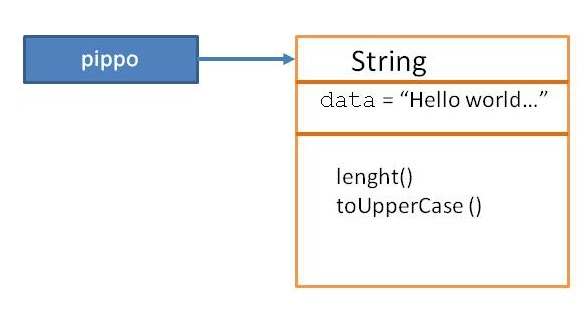
\includegraphics[scale=0.4]{images/classe.jpg}
\end{column}
\end{columns}
\begin{block}{}\footnotesize
Per il momento consideriamo un oggetto come una \textbf{black box} dotata di una \textbf{interfaccia pubblica}, che definisce il comportamento dell'oggetto, e una sua realizzazione \textbf{nascosta} (il codice dei metodi ed i loro dati)
\end{block}
\end{frame}

\subsection*{Classi}
\begin{frame}
\begin{block}{Una classe}
\begin{itemize}
\item è una \textbf{fabbrica di oggetti};
\begin{itemize}
\item gli oggetti che si creano sono \alert{esemplari}
\end{itemize}
\item specifica i metodi che si possono invocare per gli oggetti che sono esemplari di tale classe.
\item definisce i particolari della realizzazione dei metodi
\item è un contenitore di :
\begin{itemize}
\item metodi statici;
\item oggetti statici;
\end{itemize}
\end{itemize}
\end{block}
\end{frame}

\subsection*{Metodi}
\begin{frame}
\begin{block}{I metodi:}
Costituiscono l'\textCl{interfaccia pubblica} di una classe:
\begin{itemize}
\item Istruzioni valide:
\begin{itemize}
\item \texttt{String pippo = ``Hello world'';}
\item \texttt{int n = pippo.\alert{lenght()};}
\item \texttt{String river = ``Missisipi'';}
\item \texttt{String BigRiver = river.\alert{toUpperCase();}}
\end{itemize}
\item Istruzione non valida (il metodo non appartiene alla classe):
\begin{itemize}
\item \texttt{System.out\alert{.lenght();}}
\end{itemize}
\end{itemize}
\end{block}
\end{frame}

\begin{frame}
\frametitle{Metodi, parametri espliciti/impliciti}
\begin{block}{}
Alcuni metodi necessitano di \textCl{valori in ingresso} che specificano l'operazione da svolgere.
\begin{center}
\texttt{System.out.println(\textCl{pippo})}
\end{center}
\textCl{pippo} in questo caso rappresenta un parametro esplicito.
\end{block}
\begin{block}{}
Altri metodi invece non necessitano di alcun parametro. Tutte le informazioni sono memorizzate nell'oggetto corrispondente.
\begin{center}
\texttt{int n = \textCl{pippo}.length();}
\end{center}
\textCl{pippo} in questo caso è il parametro implicito.
\end{block}
\end{frame}

\begin{frame}
\frametitle{Definizione dei metodi}
\begin{block}{}
\textbf{public} \alert{void} \textCl{println(String output)}\\
\textbf{public} \alert{String} \textCl{replace(String target,String replace)}
\end{block}
\begin{block}{}
La \textbf{definizione di un metodo} inizia sempre con la sua \textbf{intestazione}, composta da:
\begin{itemize}
\item uno specificare di accesso:
\begin{itemize}
\item in questo caso è \textbf{public}, ma esiste anche la clusula \textbf{private};
\end{itemize}
\item il tipo di dati restituito dal metodo (\alert{String, void, int, double\ldots}
\item il nome del metodo (\textCl{println, replace, length})
\item un elenco di parametri, eventualmente vuoto, chiuso tra \textCl{parentesi tonde}
\begin{itemize}
\item di ogni parametro si indica il tipo e nome
\item più parametri sono separati da una virgola.
\end{itemize}
\end{itemize}
\end{block}
\end{frame}

\begin{frame}
\frametitle{Variabili oggetto}
\begin{block}{}
Una \textCl{variabile oggetto} conserva non l'oggetto stesso, ma informazioni sulla sua posizione nella memoria del computer.
Sostanzialmente è un \alert{riferimento} all'oggetto.
\end{block}
\begin{block}{}
Per definire una variabile oggetto si indica il nome della \textbf{classe} a cui l'oggetto farà riferimento la variabile,
seguito dal nome della \textCl{variabile} stessa.
\begin{center}
\alert{NomeClasse} \textCl{nomeOggetto}
\end{center}
\end{block}
\begin{block}{}
La definizione di una variabile oggetto crea un riferimento \textbf{non inizializzato}, cioè la variabile non fa riferimento ad 
alcun oggetto.
\end{block}
\end{frame}

\begin{frame}
\frametitle{Costruire oggetti: l'operatore new}
\begin{block}{}
Per \textbf{creare un oggetto} di una classe si usa l'operatore \textCl{new} seguito dal \alert{nome della classe} e da una coppia
di parentesi tonde
\begin{center}
\texttt{\textCl{new} \alert{NomeClasse}(parametri)}
\end{center}
\end{block}
\begin{block}{}
L'operatore \textCl{new} \textbf{crea un nuovo oggetto e ne restituisce un riferimento, che può essere assegnato ad una variabile}
del tipo appropiato.
\begin{center}
\textbf{NomeClasse} \alert{nomeVar} = \textCl{new} \textbf{NomeClasse(parametri)}
\end{center}
\end{block}
\end{frame}

\begin{frame}[fragile]
\begin{block}{Stringhe = Oggetti}
\begin{itemize}
\item Diversamente dai numeri, \textbf{le stringhe sono oggetti};
\begin{itemize}
\item infatti, il tipo di dati \textCl{String} inizia con la \textbf{maiuscola}
\item invece, \alert{int} e \alert{double} iniziano con la minuscola
\end{itemize}
\item Una variabile di tipo stringa quindi può essere utilizzata per invocare i metodi della classe \textCl{String};
\begin{itemize}
\item per esempio, il metodo \textCl{length} restituisce la lunghezza di una stringa, cioè \textbf{il numero di caratteri}
presenti in essa.
\end{itemize}
\end{itemize}
\end{block}
\begin{block}{}
\begin{lstlisting}
String name = "John";
int n = name.length(); // n = 4
\end{lstlisting}
\end{block}
\end{frame}

\subsubsection*{Esercitazione}
\begin{frame}
\frametitle{ESERCIZIO}
\begin{block}{}
Creare un rettangolo descritte dalle coordinate (x,y) del suo vertice in alto a sinistra e dalla larghezza e altezza.
\end{block}
\begin{block}{}
Creare un secondo rettangolo con le stesse caratteristiche del primo, e successivamente traslarlo di (15,20).
\end{block}
\begin{block}{}
Stampare le caratteristiche sia del primo che del secondo rettangolo.
\end{block}
\begin{block}{}
Potete importare la classe Rectangle, presente nel pacchetto in \alert{java.awt.Rectangle}
\end{block}
\end{frame}

\begin{frame}
\frametitle{Programmi di controllo}
Sono utilizzati per collaudare il funzionamento di una classe.
\begin{itemize}
\item Definire una nuova classe;
\item Definire in essa un nuovo metodo main;
\item Costruire oggetti all'interno del metodo main;
\item Applicare metodi agli oggetti
\item Visualizzare i risultati delle invocazioni dei metodi.
\end{itemize}
\alert{bisogna importare le classi che si vuole utilizzare.}
\begin{block}{}
Tutte le classi della libreria standard sono raccolte in \textbf{pacchetti} e sono organizzate in pacchetto o finalità. 
\texttt{java.lang} (al quale appartengono \textbf{System} e \textbf{String}) viene importata automaticamente.
\end{block}
\end{frame}

\section*{Costanti}
\begin{frame}[fragile]
\frametitle{L'uso delle costanti}
Un programma per il cambio di valuta
\begin{lstlisting}
public class Convert1{ 
    public static void main(String[] args){ 
	    double dollars = 2.35;
        double euro = dollars * 0.72;
    }
}
\end{lstlisting}
\begin{block}{}
Cosa rappresenta il \textbf{numero magico} \alert{0.72} usato per convertire i dollari in euro\ldots
\end{block}
\end{frame}
\subsection*{Uso delle costanti}
\begin{frame}[fragile]
Come è possibile definire le variabili, è opportuno definire \textbf{nomi simbolici} anche alle \textbf{costanti} utilizzate nei
programmi.
\begin{lstlisting}
public class Convert2{ 
    public static void main(String[] args){ 
        final double EURO_PER_DOLLAR = 0.72;
        double dollars = 2.35;
        double euro = dollars * EURO_PER_DOLLAR;
        double dollars2 = 3.45;
        double euro2 = dollars2 * EURO_PER_DOLLAR;
    }
}
\end{lstlisting}
\begin{block}{}
Due vantaggi principali \alert{aumento della leggibilità}; se il valore della costante deve cambiare il valore cambia in un solo 
punto.
\end{block}
\end{frame}

\begin{frame}
\frametitle{Definizione di costante}
\begin{block}{Sintassi}
\begin{center}
\texttt{\textCl{final} \textbf{nomeTipo NOME\_COSTANTE $=$ espressione}\textCl{;}}
\end{center}
\end{block}
\begin{block}{Scopo}
definire la costante \textbf{NOME\_COSTANTE} di tipo \textbf{nomeTipo} assegna il valore di \textbf{espressione}, che non potrà più
essere modificato
\end{block}
\end{frame}

\section*{Operazioni aritmetiche}
\begin{frame}
\frametitle{Operazioni aritmetiche}
\begin{block}{}
\begin{itemize}
\item L'operatore di\textbf{moltiplicazione} va sempre indicato \textbf{esplicitamente}, non può essere \textbf{sottinteso}.
\item Le operazioni di \textCl{moltiplicazione} e \textCl{divisione} \textbf{hanno la precedenza} sulle operazioni di 
\alert{addizione} e \alert{sottrazione}, cioè vengono eseguite prima.
\item \`E possibile usare \textbf{coppie di parentesi tonde} per indicare in quale oridne valutare le sotto-espressioni.
\end{itemize}
\end{block}
\begin{block}{Divisione tra interi}
\begin{itemize}
\item Quando entrambi gli operandi sono numeri \textbf{interi}, la \textbf{divisione} calcola il \alert{quoziente intero},
scartando il \textCl{resto}
\item Per avere il resto della divisione tra numeri interi è possibile utilizzare l'operatore \textCl{\%}.
\end{itemize}
\end{block}
\end{frame}

\begin{frame}
\frametitle{Combinare assegnazioni e aritmetica}
Abbiamo già visto come in Java sia possibile combinare in un unico enunciato \textCl{un'assegnazione} ed \alert{un'espressione
aritmetica che coinvolge la variabile a cui si assegnerà}
\begin{center}
\texttt{\alert{totalEuro} \textCl{=} \alert{totalEuro} + \textbf{dollars*0.72}}
\end{center}
\begin{block}{}
L'espressione di sopra è tanto comune che Java mette a disposizione delle \textbf{scorciatoie}. Infatti si può tradurre come:
\begin{center}
\texttt{\alert{totalEuro} \textCl{+=} \textbf{dollars*0.72}}
\end{center}
che esiste per tutti gli operatori aritmetici
\begin{center}
\texttt{x = x \alert{*} 2} $------>$ \texttt{x \alert{*=} 2}
\end{center}
\end{block}
\end{frame}

\begin{frame}
\frametitle{Incremento di una variabile}
\begin{block}{Incremento}
\`E l'operazione che consiste di aumentare di uno il valore di una variabile
\begin{center}
\texttt{\textbf{int counter = 0;}}\\
\texttt{\alert{counter = counter + 1}};
\end{center}
\end{block}
\begin{block}{Scorciatoie}
Anche per questo tipo di operazione Java mette a disposizione delle scorciatoie e precisamente fornisce un operatore chiamato
\textbf{incremento/decremento}
\begin{center}
\texttt{\alert{counter++;}}\\
\texttt{\alert{counter--;}}
\end{center}
\end{block}
\end{frame}  


\end{document}

